%%%%%%%%%%%%%%%%%%%%%%%%%%%%%%%%%%%%%%%%%%%%%%%%%%%%%%%%%%%%%%%%%%%%%%
% LaTeX Example: Project Report
%
% Source: http://www.howtotex.com
%
% Feel free to distribute this example, but please keep the referral
% to howtotex.com
% Date: March 2011 
% 
%%%%%%%%%%%%%%%%%%%%%%%%%%%%%%%%%%%%%%%%%%%%%%%%%%%%%%%%%%%%%%%%%%%%%%
% How to use writeLaTeX: 
%
% You edit the source code here on the left, and the preview on the
% right shows you the result within a few seconds.
%
% Bookmark this page and share the URL with your co-authors. They can
% edit at the same time!
%
% You can upload figures, bibliographies, custom classes and
% styles using the files menu.
%
% If you're new to LaTeX, the wikibook is a great place to start:
% http://en.wikibooks.org/wiki/LaTeX
%
%%%%%%%%%%%%%%%%%%%%%%%%%%%%%%%%%%%%%%%%%%%%%%%%%%%%%%%%%%%%%%%%%%%%%%
% Edit the title below to update the display in My Documents
%\title{Project Report}
%
%%% Preamble
\documentclass[paper=a4, fontsize=11pt]{article}
\usepackage[utf8]{inputenc}
\usepackage[T1]{fontenc}
\usepackage{fourier}

\usepackage[english]{babel}															% English language/hyphenation
\usepackage[protrusion=true,expansion=true]{microtype}	
\usepackage{amsmath,amsfonts,amsthm} % Math packages
\usepackage[pdftex]{graphicx}	
\usepackage{url}
\usepackage{epstopdf} % Used to import .eps files
\usepackage{float}
\usepackage[table,xcdraw]{xcolor}
\usepackage[bottom]{footmisc} % Stick footnote at bottom of page
\usepackage{xr} % Cross referencing
\externaldocument{Graph}
\setlength{\parindent}{0pt} % No indent at new paragraph

%%%% Bibliography
\usepackage[style=alphabetic,backend=bibtex]{biblatex}
\addbibresource{ch/Bibliography.bib}

%%% Custom sectioning
\usepackage{sectsty}
%\allsectionsfont{\centering \normalfont\scshape}
\allsectionsfont{\normalfont\scshape}


%%% Custom headers/footers (fancyhdr package)
\usepackage{fancyhdr}
\pagestyle{fancyplain}
\fancyhead{}											% No page header
\fancyfoot[L]{}											% Empty 
\fancyfoot[C]{}											% Empty
\fancyfoot[R]{\thepage}									% Pagenumbering
\renewcommand{\headrulewidth}{0pt}			% Remove header underlines
\renewcommand{\footrulewidth}{0pt}				% Remove footer underlines
\setlength{\headheight}{13.6pt}


%%% Equation and float numbering
\numberwithin{equation}{section}		% Equationnumbering: section.eq#
\numberwithin{figure}{section}			% Figurenumbering: section.fig#
\numberwithin{table}{section}				% Tablenumbering: section.tab#


%%% Maketitle metadata
\newcommand{\horrule}[1]{\rule{\linewidth}{#1}} 	% Horizontal rule

\title{
		%\vspace{-1in} 	
		\usefont{OT1}{bch}{b}{n}
		\normalfont \normalsize \textsc{IT University of Copenhagen} \\ [25pt]
		\horrule{0.5pt} \\[0.4cm]
		\huge Finding similar movies and frequent roles in Imdb \\
		\horrule{2pt} \\[0.5cm]
}
\author{
	\normalsize
	Andreas Precht Poulsen
	\and
	\normalsize
	Mark Thorhauge
	\and
	\normalsize
	Mikkel Hvilshøj Funch
}
\date{December 17, 2014}

%%% Begin document
\begin{document}
\maketitle
\thispagestyle{empty} % Remove numbering on first page
\setcounter{page}{0} % Make the first page number zero (not shown) so the next page starts at 1

\clearpage
\tableofcontents
\clearpage

\externaldocument{Graph}

\begingroup
\let\clearpage\relax
\section{Introduction}

\subsection{Git}
The code is available on GitHub on the following link \url{https://github.com/markthor/AlgorithmDesign}

\subsection{Project aim}
The project aims to discover interesting facts about actors, movies, etc. using algorithms, with appropriate space and time requirements, to process the data provided by IMDb\footnote{Internet Movie Database, \url{www.imdb.com}}.

\subsection{Problem statement}
\begin{itemize}
	\item The first problem is finding the most represented roles in a movie database, using a minimum amount of space. The representation of a role is defined as the percentage of times the role occurs among all roles of all movies.
	\item The second problem that the project aims to solve, is finding the Jaccard similarity of movie pairs, above a certain similarity threshold, using a minimum amount of time. The Jaccard similarity is based on a predefined subset of the movie attributes.
\end{itemize}

\subsection{Algorithmic solution}
\begin{itemize}
	\item The solution to the first problem will be based on the Misra Gries streaming algorithm. The problem is interpreted as a stream by viewing each genre of a single movie as a stream object.
	\item The solution to the second problem is calculated using locality sensitive hashing with minhashing of shingles relevant to movie data.
\end{itemize}

\subsection{Problem scope}
For the first problem, the space consumption is measured by the auxiliary space that the algorithm use. The data stream will consume some space, which is not a part of this measurement.

\subsection{Problem setting}
The data to be analysed is a dataset produced by IMDb. The data set is constructed to be loaded into a database and contains a lot of information about movies, actors, etc. However it is not all data which is relevant for the problem, so the dataset have been cleaned for all uneccesary data and a new datafile only containing roles from movies is created and used.
% !TEX root = ../preamble.tex

\section{Finding the most frequently occurring genres}
In this section, the first problem presented in section~\ref{sub:problem} is discussed, as well as different approaches to solving it.\marginpar{what problem? the problem discussed in ...}
\cite{reservoir}

\subsection{Finding heavy hitters}
Different algorithms solves the problem of finding the heavy hitters \textit{H} in a data set \textit{S}. A naïve approach is to store all distinct roles in the data set, and their respective count. A space concerned approach to finding the heavy hitters, as described in the section describing the Misra Gries algorithm, can reduce the space consumption.\marginpar{Reservoir sampling as well}

\subsection{Naïve solution}
The naïve solution stores all distinct roles in order to find the roles with a frequency above the threshold. The algorithm contains a map with every distinct role as key, and their respective count as the corresponding value. The time complexity is O(m) while the worst case space consumptions is O(m).\marginpar{Ninh was /care with time complexity}

\subsection{Reservoir Sampling}
Reservoir sampling is an algorithm that chooses \(k\) random elements from a dataset. It has a reservoir, \(Res\), of size \(k\) and a set of genres returned by the algorithm, \(R\). It holds that \(R \in Res\). Reservoir sampling can report some genres as being a heavy hitter even though it is not, i.e. the following might hold \(\exists x \left(x \in R \land x \notin H \right)\). Futhermore some heavy hitters are not included in the set of elements returned by the algorithm, i.e the following might hold \(\exists x \left(x \in H \land x \notin R \right)\).\\

Each item, \(a_i\), in \(S\) must have an equal chance of ending up in \(Res\). This is achievable by putting items \(a_1 \dots a_k\) in the reservoir. Every item after \(a_k\) has chance equal to \(\frac{1}{i}\) to be inserted in the reservoir at a random location. By doing this every item has a chance of \(\frac{1}{m}\) to be in \(Res\).

Equation~\ref{eq:one_over_m} proofs that some \(a_\ell\), \(1 \le \ell \le m\), has a chance of \(\frac{1}{m}\) to be in \(Res\), if the size of the reservoir is exactly one.
\begin{equation}
	\label{eq:one_over_m}
	\begin{split}
	Pr[a_\ell \textrm{ ends in } Res]\ 
	& = Pr[a_\ell \textrm{ is put in } Res\ \cdot \prod_{i=\ell+1}^{m} Pr[a_i \textrm{ does not replace } a_\ell] \\
	& = \frac{1}{\ell} \cdot \prod_{i=\ell+1}^{m}\left(1-\frac{1}{i}\right) \\
	& = \frac{1}{\ell} \cdot \prod_{i=\ell+1}^{m}\frac{i-1}{i} \\
	& = \frac{1}{m}
	\end{split}
\end{equation}

Generally a reservoir size of \(k\), \(k > 1\), is desirable in order to get a more precise estimate of the frequency of items in the stream. Since a proof showing that every subset of \(S\) with size \(k\) has an equal chance of being picked is along the same lines as a proof showing that every subset of \(S\) with size 2, the latter will be proofed for the sake om simplicity.
\begin{equation}
	\label{eq:one_over_m2}
	\begin{split}
	Pr[a_{\ell_1}, a_{\ell_2} \textrm{ ends in } Res]\ 
	& = \frac{2}{\ell_2} \cdot \prod_{\ell_1<i<\ell_2} \left(1- \frac{2}{i} + \frac{2}{i} \cdot \frac{1}{2}\right) \cdot \frac{2}{\ell_2} \cdot \frac{1}{2} \cdot \prod_{\ell_2 < j \le m} \left( 1 - \frac{2}{j} \right)  \\
	& = \frac{2}{\ell_1 \cdot \ell_2} \cdot \prod_{\ell_1 < i < \ell_2} \frac{i-1}{i} \cdot \prod_{\ell_2 < j \le m} \frac{j-2}{j} \\
	& = \frac{2}{\left( m - 1 \right) \cdot m} \\
	& = 1\Big/\tbinom{m}{2}
	\end{split}
\end{equation}

As seen in equation~\ref{eq:one_over_m2} every subset of \(S\) with size two has an equal chance of ending up in \(Res\). It follows that every subset of \(S\) with size \(k\) has an equal chance of being the final \(Res\).

For the algorithm to be classified as a streaming algorithm, its space consumption must be sublinear in the length of the stream. It achieves this by having the size of the reservoir fixed. To find the optimal size of the reservoir two variables are considered, \(\epsilon\) and \(\delta\). \(\epsilon\) is the error margin that one wants to achieve with probability equal to \(1 - \delta\). Considering the algorithm estimates heavy hitters it is relevant to determine the probability that the estimate is within the error margin one allows. The size of the reservoirs is dependent on these two variables. It can be calculated using the formula \(k=O\left(1/\epsilon^2\log\left(1/\delta\right)\right)\). 

Every item is only looked at once making the time complexity \(O(m)\).

%The algorithm is relevant due to its time complexity and space consumption. The time complexity is \(O(n)\), and the space consumption is \(O(\frac{t}{\alpha})\).
%As with the naïve solution, the algorithm only require a single pass through initial the dataset. After the first pass through, the algorithm counts the frequency of each item in the reservoir and reports the element if the frequency is equal to or exceeds the given threshold.
%Furthermore, it requires considerably less space than the naïve solution at the expense of guaranteeing that the result is correct. It does so by having a single reservoir array with size \(O(\frac{t}{\alpha})\), defined as mentioned above. At first the array is filled with the first \(O(\frac{t}{\alpha})\) elements in the dataset, hereafter all new elements have a chance, equal to \(\frac{t/\alpha}{n'}\) where \textit{n'} is the number of elements that have been processed at the given point in time,
% of being swapped with a random element already in the the array.
%The threshold \textit{t} is the minimum amount of times a given role, must be present in the reservoir in order to be reported as included in \(H\).\ \\
% and some heavy hitters might not  \textit{R}, is in \textit{H}, such that \(R \subseteq H\), but not necessarily \(H \subseteq R\). Therefore the algorithm might report false negatives.




 
\subsection{Misra Gries}
The Misra Gries algorithm finds heavy hitters in a data stream. It maintains a map with up to \textit{k} entries, with keys being data element identifiers. If the set of element keys in the map is denoted \textit{K}, then \(H \subseteq K\), when the algorithm has finished. The size of the map is \(k = \frac{1}{\alpha} + 1\), meaning that the fraction an element has to constitute of \textit{S} to be in \textit{H} has an inverse relation to \textit{k}.
For each element in the data stream, the map is updated. If the key of the element already exists in the map, the value is incremented by 1. Else if the size of the map is less than \textit{k}, then the element is added to the map, with a value of 1. If the element does not exist in the map and the size of the map is \textit{k}, then the value of each key is decremented by 1 and keys with value zero is removed. This decrement procedure is repeated until the size of the map is less than \textit{k} such that the element can be added to the map.

\subsubsection{Worst case example}
The soundness of the algorithm can be explained by constructing a worst case scenario. If \(H \subseteq K\), then an element occurring \(\alpha\) times must be included in the final map. Consider a stream, with an element \textit{e} being in \textit{H} with \(\alpha = 0.2\). The stream consists of 10 elements. The map has 6 entries in this example. \textit{e} occurs twice as the first two, and the most effective way of reducing the count of \textit{e} is by filling the map and presenting an element that is not yet included in the map. Because it takes 5 distinct elements to fill the map and one additional element to reduce the count of all elements, 6 elements are required to reduce \textit{e}. The stream has 10 elements and therefore this can only happen once. Therefore the count of \textit{e} is at least 1, when the algorithm terminates.\marginpar{Mangler lidt en konklusion der siger den ikke er sikker}

\subsubsection{Additional filtering}
DELETED SECTION, KEPT FOR REMEMBERING\marginpar{Den skal gerne rettes til at være single pass. False positives og false negatives er tilladte. Der skal beskrives sandsynligeheder for korrektheden}

\subsubsection{Space consumption}
The auxiliary space used by Misra Gries is \(O\left(\frac{1}{\alpha}\right)\), but as \(\alpha\) is a constant in many applications, this is regarded as constant space consumption.\marginpar{Hvornår er alpha ikke en konstant}

% !TEX root = ../preamble.tex
\section{Finding similar movies}

\subsection{Jaccard similarity}
Movie similarity is defined as Jaccard similarity of sets of a subset of movie attributes. Given two sets \textit{A} and \textit{B} the Jaccard similarity coefficient, \textit{j}, is defined as \(j = \frac{|A \cap B|}{|A \cup B|}\). \\ \\
The attributes considered when measuring similarity is title, genres, actors and directors. A set of actors is the identifiers of the actors having roles in the movie, a set of directors is the identifiers of the directors, and a set of genres is the names of the genres of the movie. The set that movie similarity is measured from is the union of all these sets as well as the title of the movie and is denoted \textit{C}.

\subsection{Min Hashing}
The purpose of Min Hashing is reducing the size the comparable movie representation, such that it still preserves its Jaccard similarity when being compared to other MinHashed objects, as well as making the representation suitable for locality-sensitive hashing.\\ \\
Min Hashing transforms \textit{C} to a signature, \(S\), which contains an integer for each hashing function used. The signature is generated by applying \textit{n} hash functions \(h_1(C), h_2(C),\ \dots\ , h_n(C)\) to the set, which produces a vector \([h_1(C), h_2(C),\ \dots\ , h_n(C)]\) of size \textit{n}, each element being the result of a hash function.\\ \\
The hash functions are defined using permutations. A permutation is a random ordering of all possible values of elements of \textit{C}, which is the union of all the sets that are to be compared. From a permutation, the hash value is computed by iterating through each element of the permutation, in the random order of the permutation. When an element is found that exists in \textit{C}, the hash function returns the index of that element in the ordering of the permutation.\\ \\
The reasoning for using Min Hash function to calculate signatures is that given two sets, \(C_1, C_2\), the probability of \(h(C_1) = h(C_2)\) is equal to the Jaccard similarity coefficient.
\begin{equation}
P(h(C_1) = h(C_2)) = \frac{|A \cap B|}{|A \cup B|}
\end{equation}
While Min Hashing produces a signature consuming significantly less space than \(C\), it stochastically preserves similarity.\\ \\
For the representation to be suitable for locality-sensitive hashing, each hash function has to be applied on each \(C_1, C_2,\ \dots\ , C_m\), producing \(m\) vectors \(S_1, S_2,\ \dots\ , S_m\), resulting in a matrix that is the input for the locality-sensitive hashing.

\begin{table}[h]
\begin{tabular}{l||l|l|l|l}
& \(S_1\) & \(S_2\) & \(S_3\) & \(S_4\) \\ \hline \hline
\(h_1(C)\) & 714 & 55 & 10034 & 183 \\ \hline
\(h_2(C)\) & 2 & 5213 & 3921 & 5213 \\ \hline
\(h_3(C)\) & 8322 & 377 & 475 & 15632
\end{tabular}
\centering
\caption{In this example, the 715'th element with index 714 of the permutation of the universal set for \(h_1(S)\) is the first element that the universal set and \(S_1\) had in common, starting from element 0.}
\end{table}

\subsection{Locality-sensitive hashing}
The purpose of locality-sensitive hashing is finding similar items, without examining each pair of items. The fundamental idea is to hash the signature of items several times, while only compare the items, of which the hash values collide. Item pairs, of which the hash value collide are called candidate pairs.\\ \\
The similarity threshold, \(t\), is the minimum similarity coefficient that a pair of items must have to be considered similar. The aim of LSH is to identify each pair with similarity greater than or equal to \(t\) as a candidate pair.\\ \\
Given a collection of signatures generated from the Min Hashing preprocessing step, each with size \(n\), the dimensions of the signature are grouped in \(b\) bands, each spanning \(r\) dimensions. The candidate pairs are found by hashing the subset of dimensions of each signature in each bands to buckets, such that two signatures with the same value in a band hashes to the same bucket. If a pair of item signatures hashes to the same bucket at least once, the items are considered candidate pairs. \\ \\

\begin{table}[h]
\begin{tabular}{l||l|l|l|l}
& \(S_1\) & \(S_2\) & \(S_3\) & \(S_4\) \\ \hline \hline
\(h_1(C)\) & \cellcolor[HTML]{FD6864} & \cellcolor[HTML]{FD6864}
 & \cellcolor[HTML]{FD6864} & \cellcolor[HTML]{FD6864} \\ \hline
\(h_2(C)\) & \cellcolor[HTML]{FD6864} & \cellcolor[HTML]{FD6864}
 & \cellcolor[HTML]{FD6864} & \cellcolor[HTML]{FD6864} \\ \hline
\(h_3(C)\) & \cellcolor[HTML]{38FFF8} & \cellcolor[HTML]{38FFF8}
 & \cellcolor[HTML]{38FFF8} & \cellcolor[HTML]{38FFF8} \\ \hline
\(h_4(C)\) & \cellcolor[HTML]{38FFF8} & \cellcolor[HTML]{38FFF8}
 & \cellcolor[HTML]{38FFF8} & \cellcolor[HTML]{38FFF8} \\ \hline
\(h_5(C)\) & \cellcolor[HTML]{9AFF99} & \cellcolor[HTML]{9AFF99}
 & \cellcolor[HTML]{9AFF99} & \cellcolor[HTML]{9AFF99} \\ \hline
\(h_6(C)\) & \cellcolor[HTML]{9AFF99} & \cellcolor[HTML]{9AFF99}
 & \cellcolor[HTML]{9AFF99} & \cellcolor[HTML]{9AFF99}
\end{tabular}
\centering
\caption{In this example the 6 rows has been divided into 3 bands with two rows each. The concrete results of the hash functions has been omitted.}
\end{table}

When the candidate pairs are found, their similarity is measured to determine whether they are actual pairs with similarity greater than or equal to \(t\). This method produces false negatives, and false positives in the sense that for some candidate pairs \(j<t\).

\subsubsection{Choosing the number of bands and rows}
The probability that two items will hash to the same bucket is a function of the similarity of the pair, the number of bands and the number of rows. A pair of items will hash to the same bucket of a band if the row values are equal, and the probability that a pair of row values are equal is \(j\). Hence the probability that a pair of items do not hash to the same bucket of one band is \(1-j^r\). The probability that the pair does not hash to the same bucket across all bands is \((1-j^r)^b\), and finally \(1-(1-j^r)^b\) is the probability that the pair is identified as a candidate pair.\\ \\
The function \(p(j) = 1-(1-j^r)^b\) is the connection between the probability that a pair is identified as a candidate pair and the similarity of the pair, \(j\). A higher number of bands clearly makes the probability larger that a pair is identified as a candidate pair, while a higher number of rows lowers this probability.\\ \\
\begin{figure}[H]
	\centering
	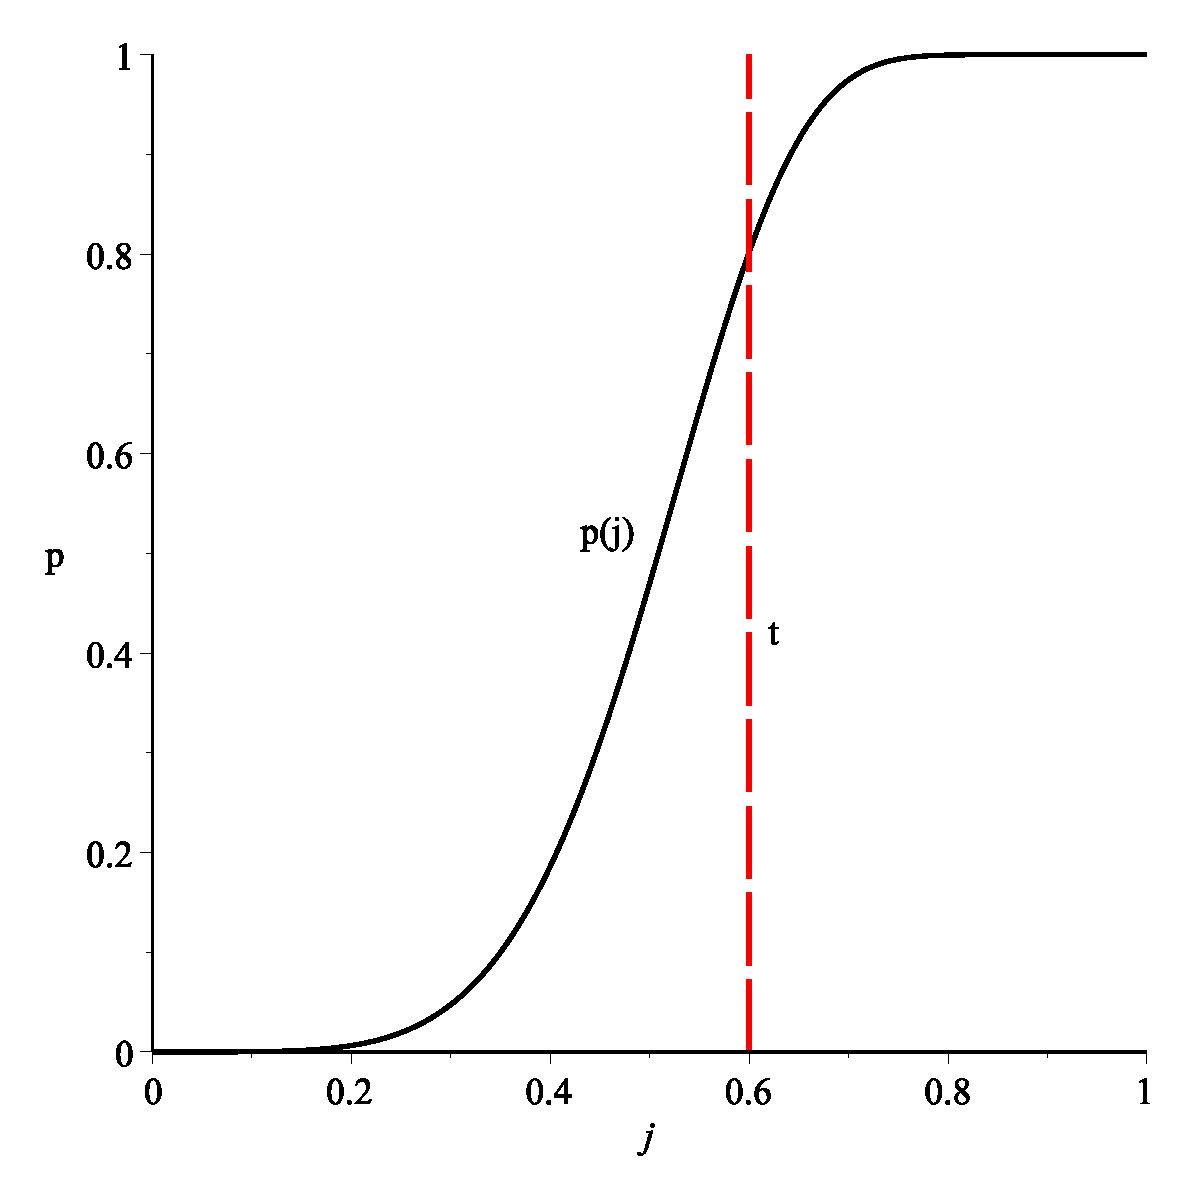
\includegraphics[width=250px]{img/pGraph.eps}
	\caption{The s-curve of \(p(j)\) with \(t = 0.6\), \(r = 5\) and \(b =20\)} 
	\label{fig:p_graph}
\end{figure}
The settings for \(b\) and \(r\) depends on the application of LSH. If the threshold is high, setting \(b\) and \(r\) to yield a low probability, might be reasonable. If the probability that a pair satisfying the threshold is identified as a candidate pair should be low, \(b\) should be increased and \(r\) lowered. Increasing b increases the fraction of false positives out of all \(n\) pairs, \(f_p\), and increasing \(r\) increases the fraction of false negatives, \(f_n\).\\ \\
To make a more precise statement on the connection between \(b\), \(r\), \(f_n\) and \(f_p\), an assumption on the distribution of item pairs has to be made. It is assumed that the distribution of items on \(j\) is continuously uniform in the interval \([0, 1]\), which is a strong assumption, because for our data set, the number of item pairs with \(j<0.2\) is much higher than the number of item pairs with \(j>0.8\).\\ \\
With a continuous uniform distribution, \(f_p\) can be estimated as the integral of \(p(j)\) from 0 to \(t\).
\[f_p = \int\limits_0^t\ p(j)\mathrm{d}j\]
To estimate \(f_n\), we subtract the entire area from \(t\) to \(1\) which is \(1-t\) with the integral of \(p(j)\) from \(t\) to \(1\).
\[f_n = (1-t)-\int\limits_t^1\ p(j)\mathrm{d}j\]

\begin{figure}[H]
	\centering
	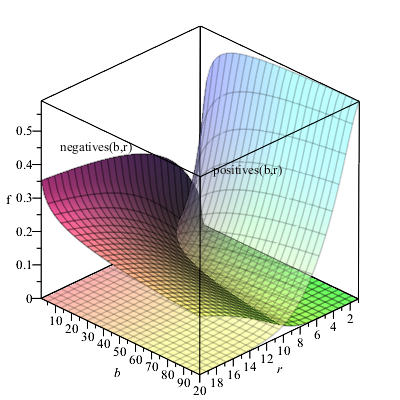
\includegraphics[width=250px]{img/falseGraph.jpg}
	\caption{The fraction of false positives or false negatives of all pairs, as a function of the number of rows and the number of bands with \(t=0.6\).}
	\label{fig:false_graph}
\end{figure}

Figure ~\ref{fig:false_graph} visualises the connection between \(b\), \(r\), \(f_n\) and \(f_p\). The connection is complicated, but it is apparent that the sum of \(f_n\) and \(f_p\) is reduced when \(b\) and \(r\) are increased.

% !TEX root = ../preamble.tex
\section{Implementation}

\subsection{Data cleaning}
The data used for problem one, containing the roles and the string describing the actual role has superfluous information, e.g. the id of the actor, the id of the movie. The string describing the role can for instance contain information defining what specific policeman it was. In order to generalise the roles such information is removed, e.g. there is no difference between policeman \#1 and policeman \#2 in the cleaned dataset. Additionally unspecified roles are deleted. As an example multiple people has had a role playing themselves. Such a role is defined as “Themselves” in the dataset, which is very general and not an actual role, hence these are deleted. Other similar roles, e.g. "himself", "herself", "extra" or "additional" are removed as well. Some roles define which year the role was from. This information is also removed. Finally, many of the string describing the roles are empty. These entries are deleted.

\subsubsection{Movie wrangling}
The data used for problem two has to be wrangled in order to fit the problem. The movie data considered when comparing movies are the following:
\begin{itemize}
\item Title
\item Director ids
\item Actor ids
\item Genres as strings
\end{itemize}
The movies are loaded in RAM and the attributes are stored in sets. The sets that is used as an input to jaccard similarity coefficient calculation is the union of all the sets. Movies with less than \(x\) elements in the union set is not used as input for similarity sensitive hashing.

\subsection{Practical space consumption}
The following logarithmic graph is the number of map entries used by Misra Gries, reservoir sampling and the naive solution based on the concrete data set. The vertical axis is space consumption and the horizontal axis is \(\alpha\). Only the naïve solution is dependent on the size of the concrete example and not on \(\alpha\). The reservoir sampling algorithm is linear dependent on the threshold.
\begin{figure}[H]
	\centering
	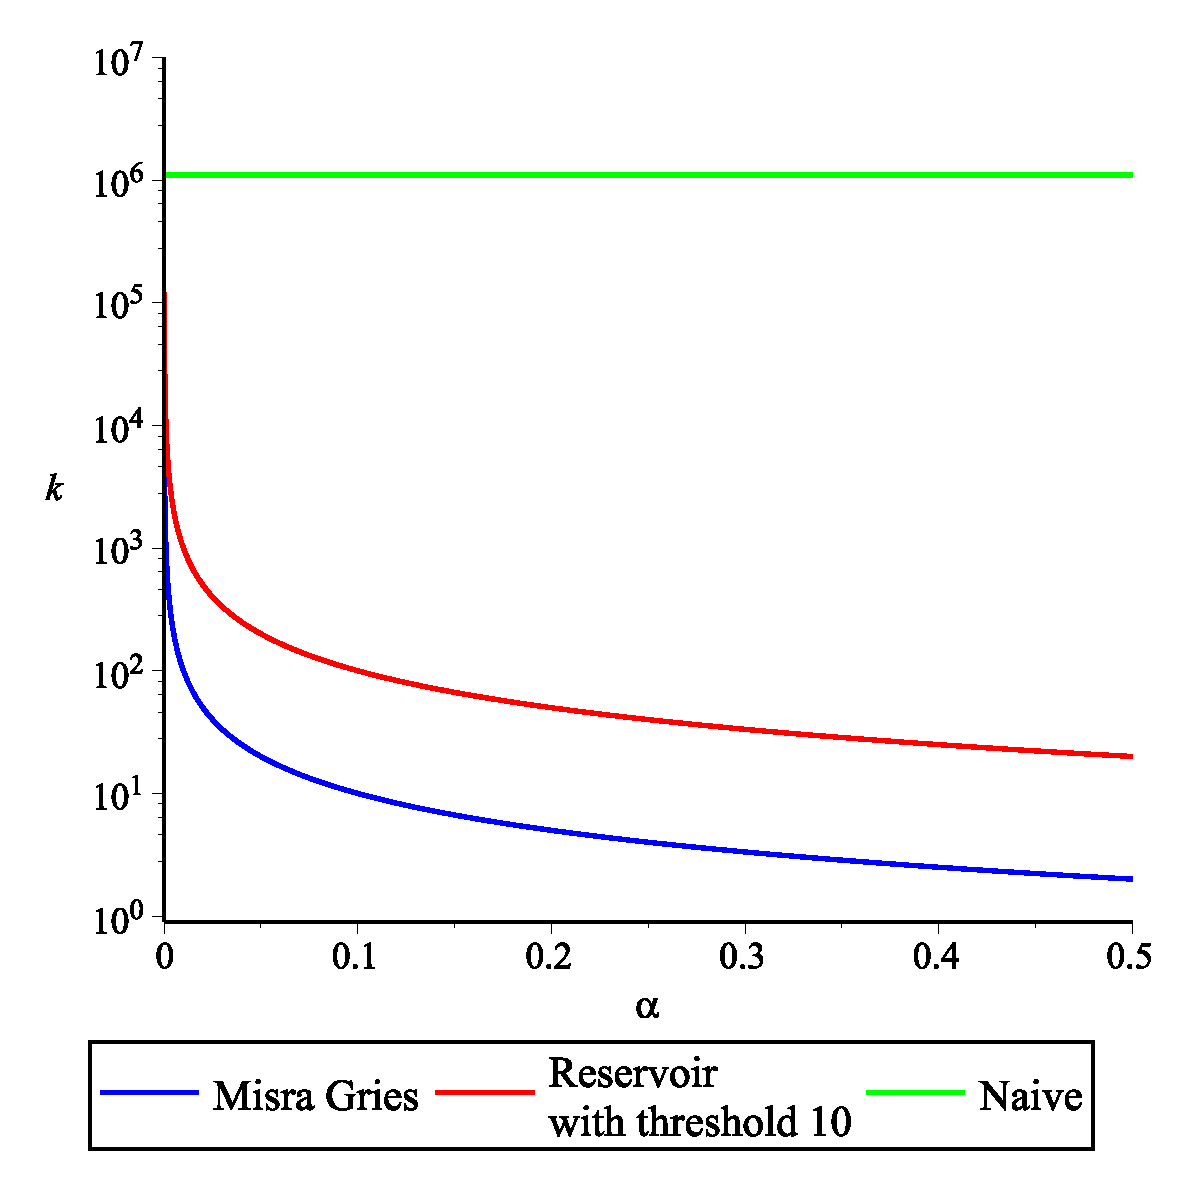
\includegraphics[width=290px]{img/streamingMemoryGraph.eps}
	\caption{Space consumption}
	\label{fig:space_consumption}
\end{figure}
As seen in figure~\ref{fig:space_consumption} the space used by the naïve solution is 1000 times as large as the space used by Misra Gries and reservoir sampling. when looking for elements in Hwith =0.001. The size of the data stream is approximately 2.3 million.

\subsection{Applications}
Locality-sensitive hashing have a wide range of applications where it proves to be relevant and quite popular.\cite{mikkel1}\cite{mikkel2} Here is mentioned a small part of the applications.  \\
It is specifically widely used in the field of "Nearest neighbor search"; data compression, databases, data mining, image- and video-databases, machine learning, pattern recognition, etc. all use locality-sensitive hashing and especially when the dimensions of the problem are high, is the algorithm efficient.
It is also used in combination with the "k-nearest neighbors algorithm", also known as "k-nn", which is widely used, among others, in the fields of machine learning and recommender systems such as those used by Netflix\footnote{\url{www.netflix.com}} and Pandora\footnote{\url{www.pandora.com}}. Applications doing video- and Audio-fingerprinting, such as Shazam\footnote{\url{www.shazam.com}} and Youtube\footnote{\url{www.youtube.com}} can also use the algorithm in order to find music tracks that sounds most alike, as done by Shazam, or to automatically remove videos containing illegal footage, as done by Youtube.


\section{Conclusion}
The problem of finding the most represented roles has been solved using Misra Gries and reservoir sampling. Both solutions uses a sublinear amount of space, but they introduce different problems. Misra Gries returns a large amount of false positives for the concrete problem instance, which makes it difficult to tell exactly which roles that are the most represented for a small \(\alpha\). Reservoir sampling uses less space if a certain uncertainty can be accepted.\\ \\
The problem of finding the most similar movies has been solved using locality-sensitive hashing. The algorithm successfully reduces the running time to less than quadratic. However the movie data from the data set is not high-dimensional, which results in the number of permutations for Min Hashing being low. Therefore LSH is left with a low number of bands and rows, which is a sub-optimal setting. In a problem setting with a higher number of dimensions, the solution would yield more impressive result.

\appendix
% !TEX root = ../preamble.tex
\section{Graphs}\label{sec:graph}
\begin{figure}[H]
	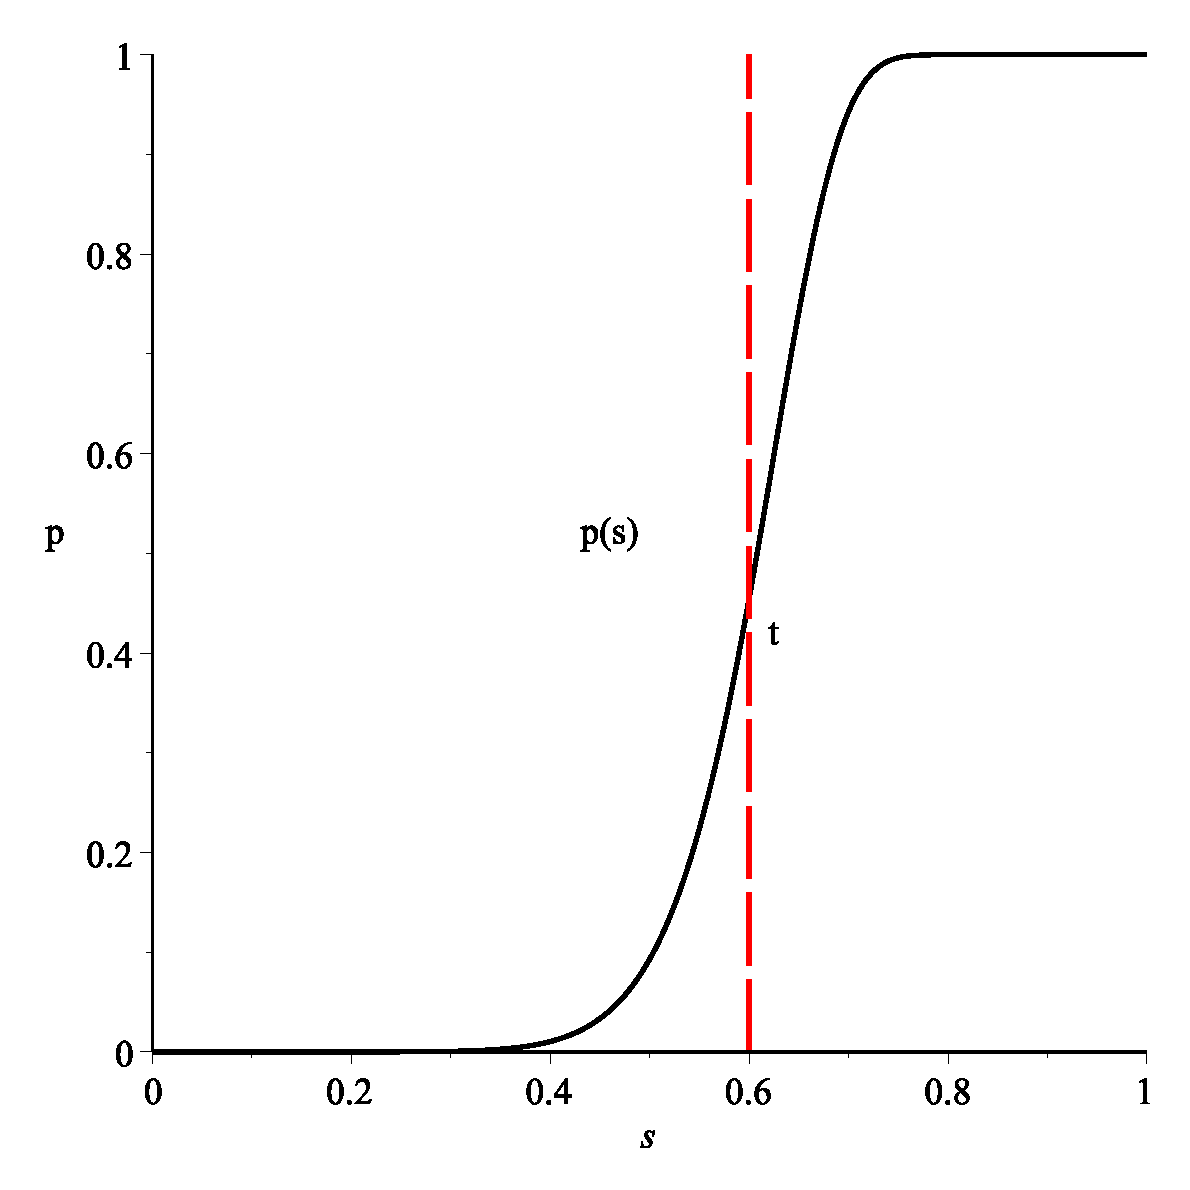
\includegraphics[width=290px]{img/pGraphGood.eps}
	\label{fig:p_graph_good}
\end{figure}
% !TEX root = ../preamble.tex

\section{Test runs of similarity search}
These are the results of 5 test runs using threshold \textit{0.6} \\ \\
Run 1, threshold = 0.6 \\
Return 1 movie: \\
Movies "Avril" and "Coster Bill" have jaccard similarity: 0.64. \\\\
Run 2, 3, 4 and 5, threshold = 0.6 \\
Return 0 movies. \\

Because of the low amount of results we, temporarily lowered the threshold to \textit{0.4} and made 5 new test runs: \\ \\
Run 1, threshold = 0.4 \\
Return 2 movies: \\
Movies "Brittany’s Foot Tease" and "Buuel" have jaccard similarity: 0.5. \\
Movies "38" and "Bruce Springsteen \& the E Street Band: Live in Barcelona" have jaccard similarity: 0.44. \\ \\
Run 2 \\
Movies "All I Desire" and "Apartment for Peggy" have jaccard similarity: 0.6. \\
Movies "Cndida” and "Crcel de Cananea” have jaccard similarity: 0.43. \\ \\
Run 3, threshold = 0.4. \\
Movies "Bodily Harm" and "Castro Laboreiro" have jaccard similarity: 0.43. \\
Movies "Cndida and "Crcel de Cananea” have jaccard similarity: 0.43. \\
Movies "Atta Boy’s Last Race" and "Bodily Harm" have jaccard similarity: 0.42. \\
Movies "Ablution" and "Accadde tra le sbarre" have jaccard similarity: 0.49. \\ \\
Run 4, threshold = 0.4. \\
Movies "Awal el shahir" and "Awal hub" have jaccard similarity: 0.5. \\
Movies "Cndida” and "Crcel de Cananea” have jaccard similarity: 0.43. \\ \\
Run 5, threshold = 0.4. \\
Movies "Avci" and "Cento cavalieri” have jaccard similarity: 0.41. \\
Movies "Apartment for Peggy" and "Chyortova dyuzhyna" have jaccard similarity: 0.42. \\
Movies "After School Special" and "Blond: Eva Blond! - Der Zwerg im Schliefach" have jaccard similarity: 0.47. \\
Movies "Dai nu qing hen" and "Dai Nippon teikoku" have jaccard similarity: 0.44. \\
Movies "Brittany’s Foot Tease" and "Buuel" have jaccard similarity: 0.5. \\
Movies "Avril" and "Coster Bill" have jaccard similarity: 0.64. \\

From the limited amounts of test that we have run, it is clear that quite a few of all the actual movie pairs above the threshold is found at every run. The amount of candidate pairs is extremely wide, with the lowest values being under 1000 and the highest values being above 70000.



\endgroup

\clearpage % Force bibliography on new page
\printbibliography

%%% End document
\end{document}